\section{Обработка табличных данных. Часть 2.}

\textbf{Задание:} Ваш выбор: Все нечетные столбцы заменить столбцом X. 
(Нумерация столбцов массива начинается с нуля.)

Создано окно приложения, содержащее 5 элементов \verb|Button|, 3 элемента \verb|DataGridView| 
и 5 элементов \verb|Label|. 
Для отображения сообщений об ошибках в окно добавлен элемент \verb|ErrorProvider|. 
Вид окна представлен на рисунке \ref{fig:task5_form}.
\begin{figure}[H]
    \centering
    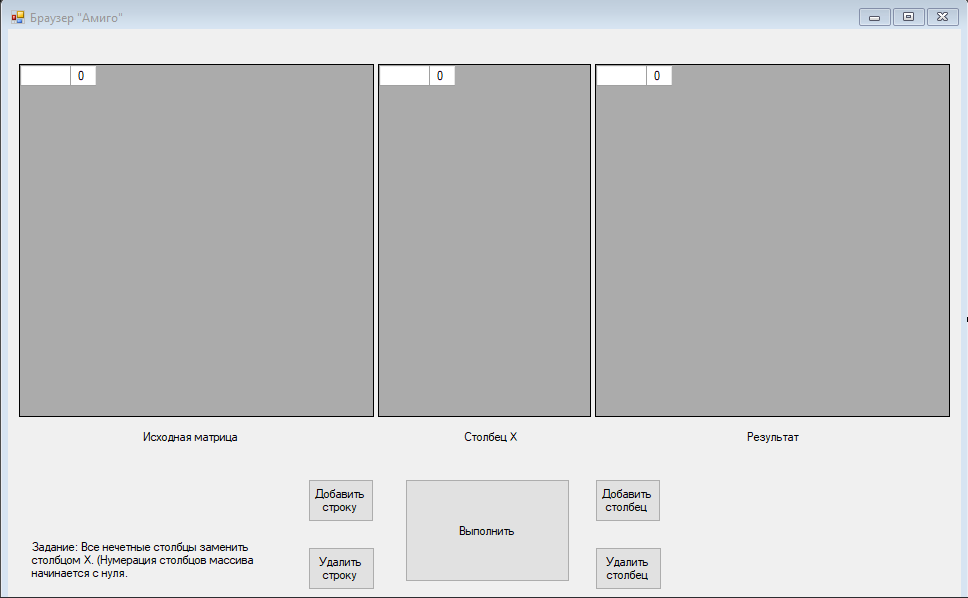
\includegraphics[scale=0.6]{task5/form.png}
    \caption{Внешний вид формы программы}
    \label{fig:task5_form}
\end{figure}
У элементов изменены значения некоторых атрибутов. 
Значения измененных атрибутов представлены в таблице \ref{table:params5}.
\begin{table}[H]
    \small
    \caption{Значения атрибутов элементов в приложении <<Обработка табличных данных. Часть 2.>>}
    \begin{tabular}{|l|l|}\hline
    Наименование атрибута & Значение\cr\hline
    \multicolumn{2}{|l|}{Для формы}\cr\hline
    \verb"Text" & \verb"Браузер "Амиго""\cr\hline
    \verb"FormBorderStyle" & \verb"FixedSingle"\cr\hline
    \verb"MaximizeBox" & \verb"False"\cr\hline
    \multicolumn{2}{|l|}{Для первой надписи}\cr\hline
    \verb"(Name)" & \verb"taskLabel"\cr\hline
    \verb"Text" & \verb"Задание: Все нечетные столбцы заменить столбцом X."\cr\hline
    \multicolumn{2}{|l|}{Для второй надписи}\cr\hline
    \verb"(Name)" & \verb"initLabel"\cr\hline
    \verb"Text" & \verb"Исходная матрица"\cr\hline
    \multicolumn{2}{|l|}{Для третьей надписи}\cr\hline
    \verb"(Name)" & \verb"xLabel"\cr\hline
    \verb"Text" & \verb"Столбец X"\cr\hline
    \multicolumn{2}{|l|}{Для четвертой надписи}\cr\hline
    \verb"(Name)" & \verb"resultLabel"\cr\hline
    \verb"Text" & \verb"Результат"\cr\hline
    \multicolumn{2}{|l|}{Для кнопки "Выполнить"}\cr\hline
    \verb"(Name)" & \verb"btnCalc"\cr\hline
    \multicolumn{2}{|l|}{Для кнопки добавления ряда}\cr\hline
    \verb"(Name)" & \verb"btnAddRow"\cr\hline
    \verb"Text" & \verb"Добавить"\cr\hline
    \multicolumn{2}{|l|}{Для кнопки удаления ряда}\cr\hline
    \verb"(Name)" & \verb"btnRemoveRow"\cr\hline
    \verb"Text" & \verb"Удалить"\cr\hline
    \multicolumn{2}{|l|}{Для кнопки добавления столбца}\cr\hline
    \verb"(Name)" & \verb"btnAddColumn"\cr\hline
    \verb"Text" & \verb"Добавить"\cr\hline
    \multicolumn{2}{|l|}{Для кнопки удаления столбца}\cr\hline
    \verb"(Name)" & \verb"btnRemoveColumn"\cr\hline
    \verb"Text" & \verb"Удалить"\cr\hline
    \multicolumn{2}{|l|}{Для обработчика ошибок}\cr\hline
    \verb"(Name)" & \verb"errorProvider1"\cr\hline
    \end{tabular}
    \label{table:params5}
\end{table}

После запуска приложения на экране появляется окно (см. рисунок \ref{fig:exec5})
\begin{figure}[H]
    \centering
    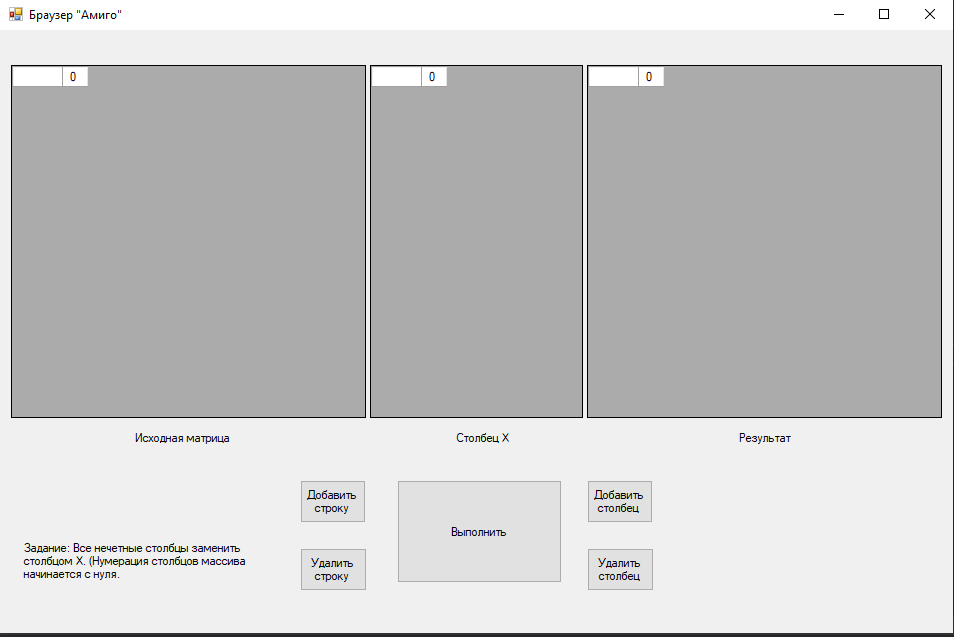
\includegraphics[scale=0.6]{task5/exec.png}
    \caption{Скриншот запуска программы}
    \label{fig:exec5}
\end{figure}
При вводе целого числа после нажатия кнопки в поле вывода приводится
результат вычисления суммы в заданном интервале (см. рисунок \ref{fig:result5}).
\begin{figure}[H]
    \centering
    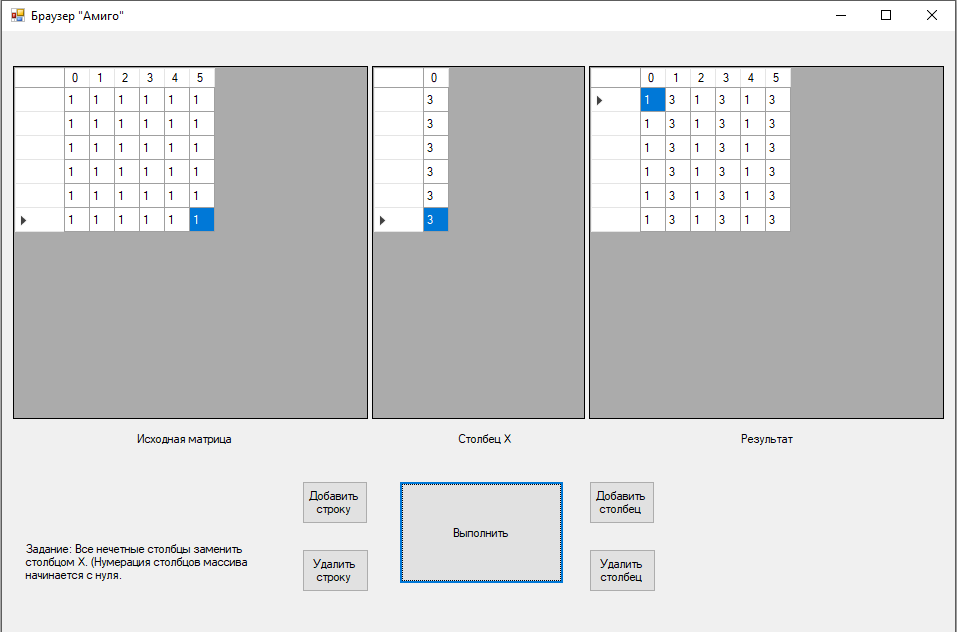
\includegraphics[scale=0.6]{task5/result.png}
    \caption{Результат работы}
    \label{fig:result5}
\end{figure}
Ввод некорректных значений обрабатывается элементом \verb|ErrorProvider| и 
сопровождается сообщением об ошибке (см. рисунок \ref{fig:error5} )
\begin{figure}[H]
    \centering
    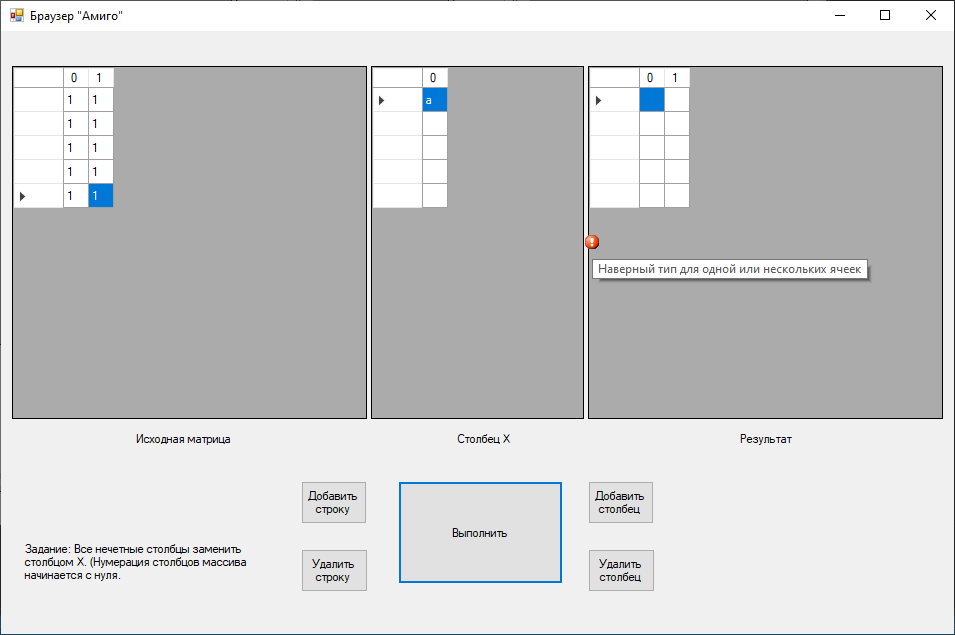
\includegraphics[scale=0.45]{task5/error.png}
    \caption{Сообщение об ошибке}
    \label{fig:error5}
\end{figure}
Полный код программы приведен в приложении \ref{app:repos}.